\documentclass[newPxFont]{beamer}
%\documentclass[handout]{beamer} % Раздаточный материал (на слайдах всё сразу)
%\documentclass[aspectratio=169]{beamer} % Соотношение сторон


\usetheme{LTX}

%-=-=-=-=-=-=-=-=-=-=-=-=-=-=-=-=-=-=-=-=-=-=-=-=
%        LOADING PACKAGES
%-=-=-=-=-=-=-=-=-=-=-=-=-=-=-=-=-=-=-=-=-=-=-=-=
\usepackage{amsmath,amsfonts,amssymb,amsthm,mathtools}  % Тут мы подключаем пакеты для математики!
\usepackage{wasysym}
%%%%%%%%%%%%%%%%%%%%%%%% Шрифты %%%%%%%%%%%%%%%%%%%%%%%%%%%%%%%%%

\usepackage{fontspec}         % пакет для подгрузки шрифтов
\setmainfont{HelveticaNeueCyr}   % задаёт основной шрифт документа

% why do we need \newfontfamily:
% http://tex.stackexchange.com/questions/91507/
\newfontfamily{\cyrillicfonttt}{HelveticaNeueCyr}
\newfontfamily{\cyrillicfont}{HelveticaNeueCyr}
\newfontfamily{\cyrillicfontsf}{HelveticaNeueCyr}
% Иногда тех не видит структуры шрифтов. Эти трое бравых парней спасают ситуацию и доопределяют те куски, которые Тех не увидел.

% \usepackage{unicode-math}     % пакет для установки математического шрифта
% \setmathfont{Asana Math}      % шрифт для математики

\usepackage{polyglossia}      % Пакет, который позволяет подгружать русские буквы
\setdefaultlanguage{russian}  % Основной язык документа
\setotherlanguage{english}    % Второстепенный язык документа

%%% Работа с картинками
\usepackage{graphicx}  % Для вставки рисунков
\graphicspath{{images/}{images2/}}  % папки с картинками
\setlength\fboxsep{3pt} % Отступ рамки \fbox{} от рисунка
\setlength\fboxrule{1pt} % Толщина линий рамки \fbox{}
\usepackage{wrapfig} % Обтекание рисунков текстом

%%% Работа с таблицами
\usepackage{array,tabularx,tabulary,booktabs} % Дополнительная работа с таблицами
\usepackage{longtable}  % Длинные таблицы
\usepackage{multirow} % Слияние строк в таблице

%%% Программирование
\usepackage{etoolbox} % логические операторы

%%% Другие пакеты
\usepackage{multicol} % Несколько колонок

%%% Картинки
\usepackage{tikz} % Работа с графикой
\usepackage{pgfplots}
\usepackage{pgfplotstable}


\usepackage{xcolor}
\usepackage{hyperref}
\hypersetup{				
    unicode=true,           % позволяет использовать юникодные символы
    colorlinks=true,       	% true - цветные ссылки, false - ссылки в рамках
    urlcolor=blue,          % цвет ссылки на url
    linkcolor=red,          % внутренние ссылки
	hyperindex=true         % сделать ли ссылку кликабельной?
	breaklinks=true         % если ссылка не умещается в одну строку, разбивать    
	                        % ли ее на две части?
}
\usepackage{verbatim}
\usepackage{fancyvrb}
\usepackage{mdframed}

 
\usepackage{chronology}

\renewcommand{\event}[3][e]{%
  \pgfmathsetlength\xstop{(#2-\theyearstart)*\unit}%
  \ifx #1e%
    \draw[fill=black,draw=none,opacity=0.5]%
      (\xstop, 0) circle (.2\unit)%
      node[opacity=1,rotate=45,right=.2\unit] {#3};%
  \else%
    \pgfmathsetlength\xstart{(#1-\theyearstart)*\unit}%
    \draw[fill=black,draw=none,opacity=0.5,rounded corners=.1\unit]%
      (\xstart,-.1\unit) rectangle%
      node[opacity=1,rotate=45,right=.2\unit] {#3} (\xstop,.1\unit);%
  \fi}%

\title{Уютный факультатив по \LaTeX}
\subtitle{Введение в \LaTeX}
\date{\today}

\begin{document}

\begingroup
\setbeamercolor{background canvas}{bg = LTXDarkGrey}
\begin{frame}[plain]
\begin{center}
\LARGE{\color{red}{ВНИМАНИЕ!}}
\end{center}
\color{white}{ДАННЫЙ КУРС СОДЕРЖИТ БОЛЬШОЕ КОЛИЧЕСТВО РАЗНООБРАЗНОГО КОДА И ЗАДАНИЙ ДЛЯ САМОСТОЯТЕЛЬНОГО РЕШЕНИЯ.\\ НА ПЕРВЫЙ ВЗГЛЯД ОН МОЖЕТ ПОКАЗАТЬСЯ СЛОЖНЫМ И ТРАВМИРОВАТЬ НЕПОДГОТОВЛЕННУЮ ПСИХИКУ. \\ ТАКЖЕ ОН СОДЕРЖИТ БОЛЬШОЕ КОЛИЧЕСТВО НЕУДАЧНЫХ ШУТОК И НЕУМЕСТНЫХ ОТСЫЛОК. \\ В СВЯЗИ С ЭТИМ КУРС НЕ РЕКОМЕНДУЕТСЯ ПРОСЛУШИВАТЬ \ldots НИКОМУ.}
\end{frame}
\endgroup 

 \maketitle
 
\begin{frame}
\frametitle{Идеология курса}
\begin{itemize}
\item 8 лекций и 8 семинаров 
\item лекция --- я рассказываю какие-то вещи
\item что-то неясно $\Rightarrow$ \alert{СПРОСИ}
\item семинар --- мы закрепляем эти вещи
\item на семинаре присутствуют 4-5 человек, которые хорошо знают \LaTeX{} и помогают вам
\item есть проблема $\Rightarrow$ \alert{зови одного из нас}
\item для зачёта надо сдать 70\% домашек
\end{itemize} 
\end{frame} 


\begin{frame}
\frametitle{Повестка курса}
\begin{enumerate}
\item Обо всём и ни о чём! Мотивация, математика.
\item Шрифты, рисунки и таблицы.
\item Оформление докумена в целом.
\item Список литературы. Bib\LaTeX{}. Сложные документы.
\item Графика, TikZ, Geogebra. Свои команды и макросы.
\item Преамбула для души и для ГОСТ. Bib\LaTeX{-gost}.
\item Связка R и \LaTeX{}. Автоматизация создания документов.
\item Презентации в \LaTeX{} - большая боль или чувство стиля?
\end{enumerate}
\end{frame} 


\begin{frame}
\frametitle{Куда идти за мудростью}

У нашего курса есть страничка на Github! Многие из вас уже были там и видели, что там много разной мудрости.
\vspace{1cm}

\begin{block}{Страничка курса:}
\vspace{3mm}
\centerline {\url{https://fulyankin.github.io/LaTeX/}} 
\vspace{3mm}
\end{block}
\end{frame}


\begin{frame}
\frametitle{Что это вообще такое ?} 
\alert{TeX} --- это созданная американским математиком и программистом Дональдом Кнутом система для верстки текстов с формулами. 

\centering 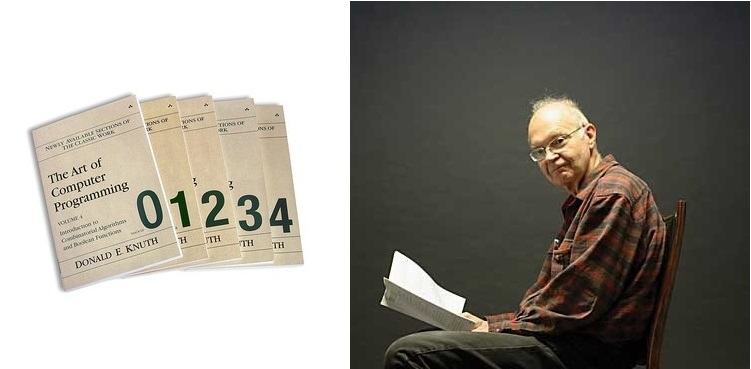
\includegraphics[scale=0.5]{knut.jpg}\\
\end{frame} 


\begin{frame}
\frametitle{Почему \LaTeX{}?} 
\begin{itemize}
\item Он позволяет делать красивые документы
\item Особенно документы с формулами
\item Он был создан учёными для учёных
\item Большое и активное комьюнити, у которого всегда можно попросить о помощи
\item Он уютный!
\item Многие вещи, связанные с оформлением автоматизированы, что позволяет думать о содержании
\item Огромное количество различных пакетов и расширений в свободном доступе
\end{itemize}
\end{frame}


\begin{frame}
\frametitle{Откуда появился \LaTeX{}?} 
\begin{columns}
\begin{column}{.48\linewidth}
\centering 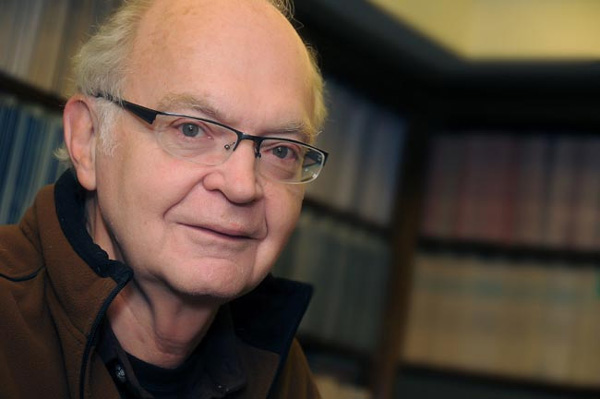
\includegraphics[scale=0.2]{DK.jpg}\\
\mbox{ } \\
Дональд Кнут создал в 1978 году программу \TeX.		
\end{column}

\begin{column}{.48\linewidth}
\centering Лесли Лэмпорт создал в 1984 году макропакет \LaTeX. \\
\mbox{ } \\
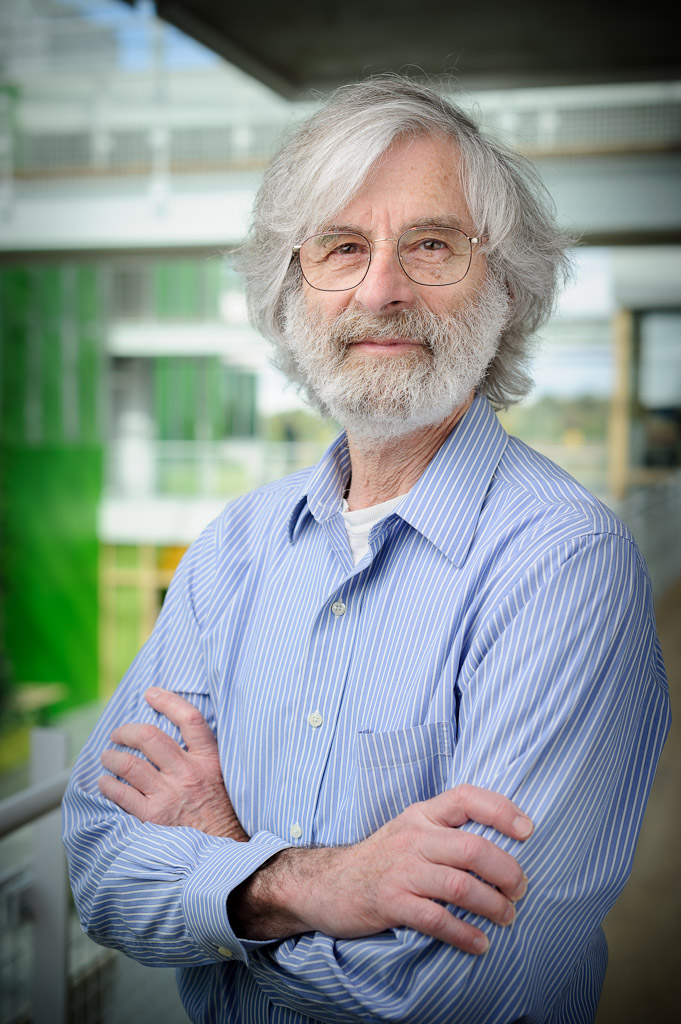
\includegraphics[scale=0.4]{LL.jpg}		
\end{column}
\end{columns}
\end{frame}


\begin{frame}{Движки}
\centering 
	\begin{tabulary}{\textwidth}{JcJ}
		\toprule
			движок			& рождение & отличия	\\[0.25em]
		\midrule
		\TeX{}				    & 1978 & начало пути  \\[0.25em]
		\LaTeX{}				& 1984 & расширение, упрощение \\[0.25em] 
		\midrule

		pdf\LaTeX{}				& 2000 & сборка не dvi, а сразу pdf  \\[0.25em]
		Xe\LaTeX{}				& 2004 & юникод, куча шрифтов   \\[0.25em]
		Lua\LaTeX{} 		    & 2007 & язык Lua + Xe\LaTeX     \\[0.25em]
		\midrule
		bib\TeX{}				& 1985 &  удобная библиография  \\[0.25em]
		bib\LaTeX{} (biber)		& 2010 &  юникод, ряд улучшений    \\[0.25em]
		\bottomrule
	\end{tabulary}
	
	\mbox{ }

	\href{https://habrahabr.ru/post/114610/}{Статья про движки на хабре}
\end{frame}


\begin{frame}{О правильном софте}
\begin{columns}
\begin{column}{.48\linewidth}

\includegraphics[width=0.5\linewidth]{RStudio-Ball.png}\\
\mbox{ } \\

\includegraphics[width=0.9\linewidth]{Python-logo.png}\\
\end{column}


\begin{column}{.48\linewidth}

\includegraphics[width=0.6\linewidth]{julia-logo.png}	
\mbox{ } \\

\includegraphics[width=0.9\linewidth]{c-vs-cpp.png}
\end{column}
\end{columns}
\end{frame}


\begin{frame}{Популярность языков программирования}
\centering 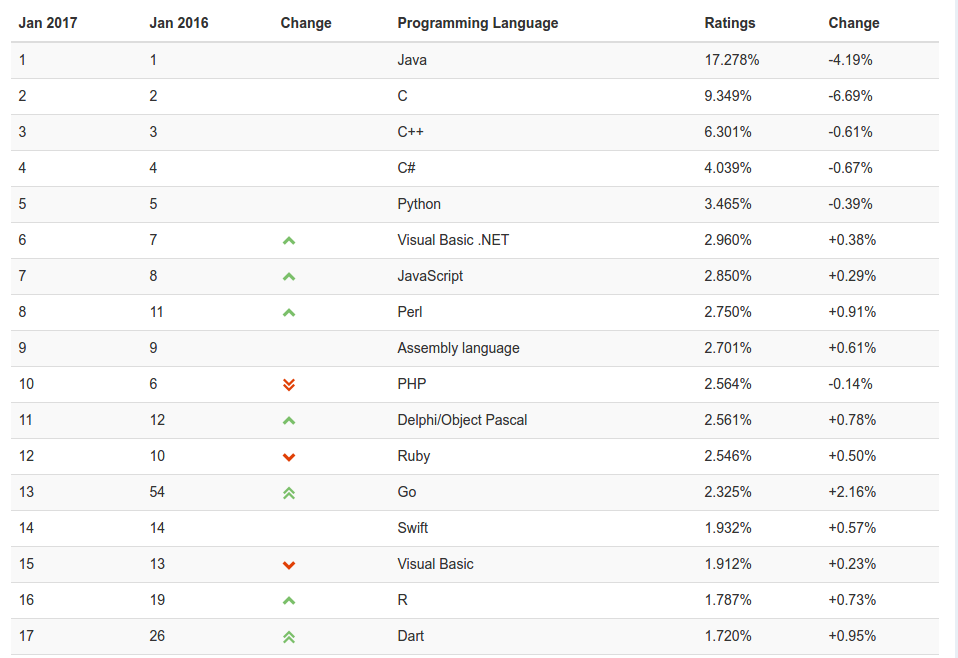
\includegraphics[width=0.7\linewidth]{lang.png}\\
\vspace{0.2cm}
Подробнее на \centerline {\url{http://www.tiobe.com/tiobe-index/}} 
\end{frame}


\begin{frame}{Самый важный язык}
\centering 
\includegraphics[width=\linewidth]{english.jpg}\\
\end{frame}


\begin{frame}{<<How to \ldots>> а также <<Error: \ldots>>}
\centering 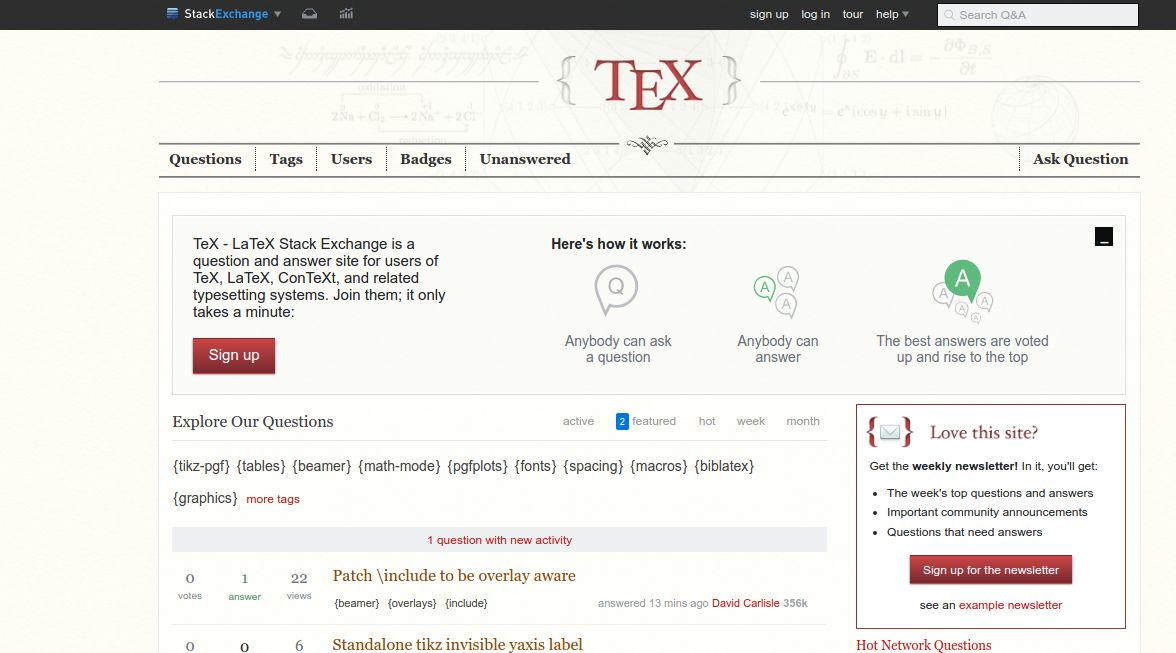
\includegraphics[width=\linewidth]{texexchan.png}\\
\end{frame}


\begin{frame}{Мой рук}
\centering 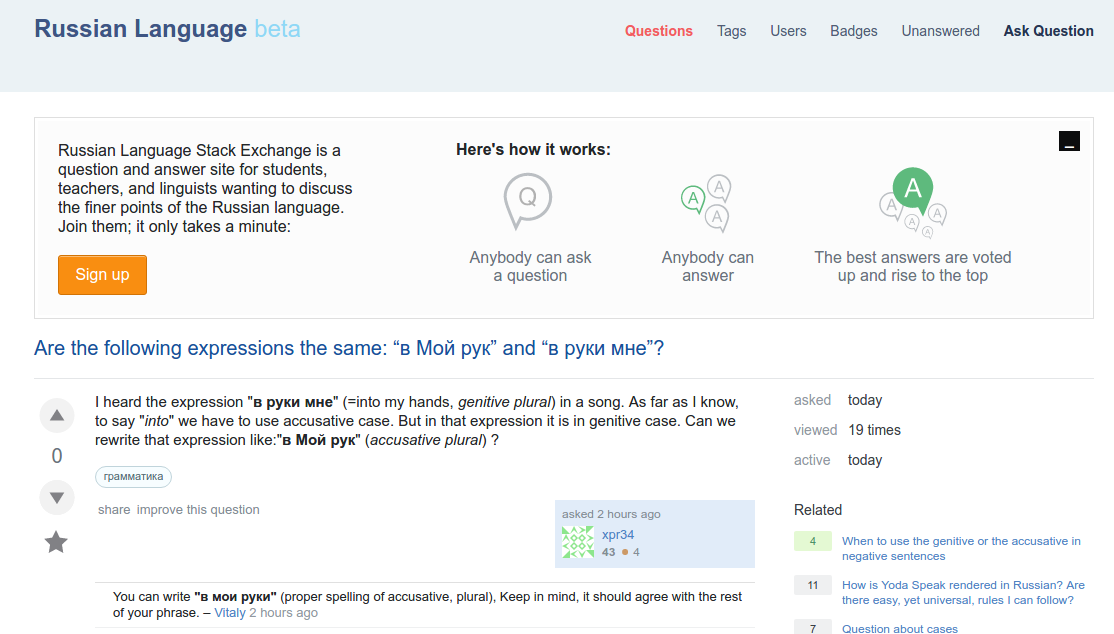
\includegraphics[width=\linewidth]{russia.png}\\
\end{frame}


\begin{frame}{Мемы про Stack Overflow} 
\begin{columns}
\begin{column}{.48\linewidth}

\includegraphics[width=\linewidth]{googling.jpg}\\
\end{column}


\begin{column}{.48\linewidth}
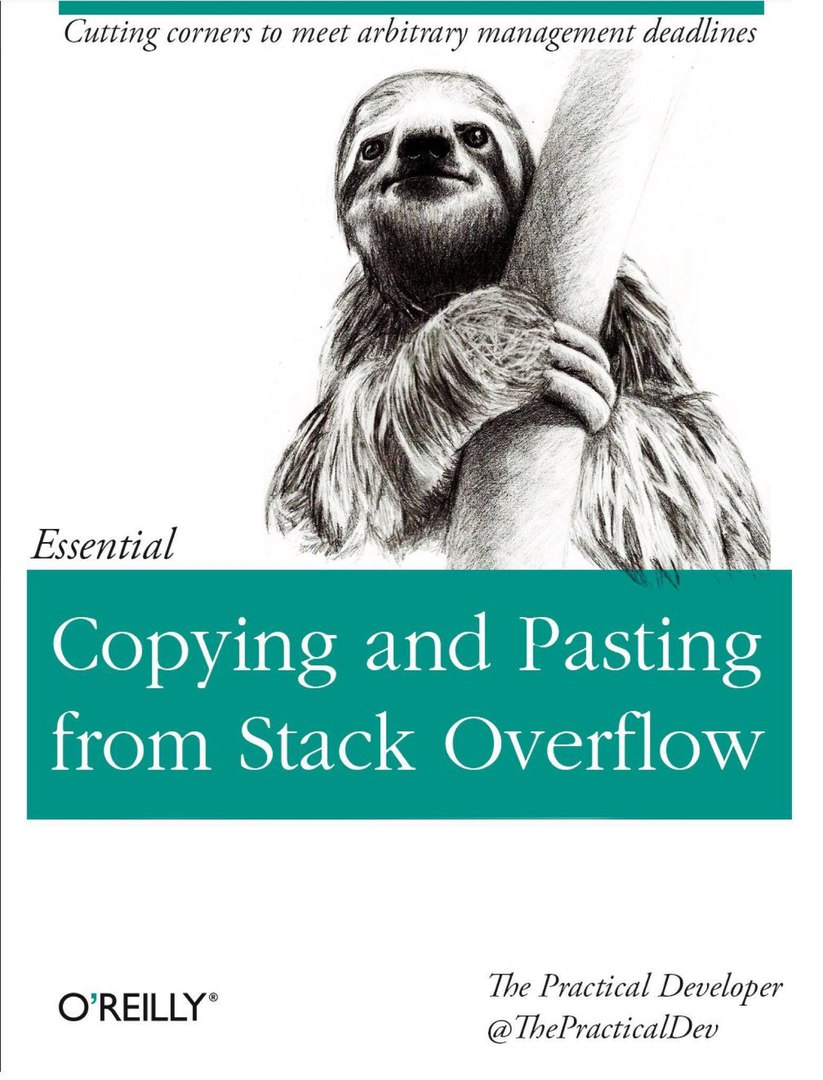
\includegraphics[width=\linewidth]{copypast.jpg}\\	
\end{column}
\end{columns}
\end{frame}


\begin{frame}
\frametitle{Особенности \LaTeX}
\LaTeX{} не WYSIWYG (What You See Is What You GET)
В WYSIWYG системах что автор видит на экране, то и получается на печати.

\mbox{ } 

\LaTeX{} WYSIWYM (What You See Is What You \alert{MEAN})
\LaTeX{} сам позаботится об оформлении, вам остаётся только думать о содержании!
\end{frame}



\begin{frame}[fragile]
\frametitle{Как это работает?}
Вы пишите свой текст с различными \alert{командами}, описывающими структуру текста, а \LaTeX{} преобразует их в красиво отформатированный pdf-документ!

\begin{mdframed}[backgroundcolor=LTXLightGreen]
В Португалии \verb|\textbf|\{дождь\} является \verb|\textit|\{причиной\}  не выходить на работу.
\end{mdframed}

\centering
   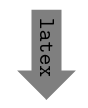
\includegraphics[scale=0.3]{fuc.png}%}

\begin{mdframed}[backgroundcolor=LTXLightGreen] 
В Португалии \textbf{дождь} является \textit{причиной} не выходить на работу.
\end{mdframed}   
\end{frame}

\begin{frame}[fragile]
\frametitle{Ещё примеры работы \LaTeX{}!} 

\begin{tabular}{p{5.5cm}p{4cm}}
\vspace{10mm} \verb|includegraphics[scale=0.15]{doge.png}| &  \begin{center} 
\includegraphics[scale=0.15]{doge.png} \end{center}
\end{tabular}
\begin{tabular}{p{5.5cm}p{4cm}}
\centering \verb|$\alpha^{x}+\sigma_{t}$| & \centering  $\alpha^{x}+\sigma_{t}$
\end{tabular}
\begin{tabular}{p{6.5cm}p{4cm}}
\begin{verbatim}
\begin{enumerate}
\item Чай
\item Молоко
\end{enumerate}
\end{verbatim} 
& \vspace{6mm} \begin{center}
\begin{enumerate}
	\item Чай
	\item Молоко
\end{enumerate}	 
\end{center} 
\end{tabular}
\end{frame}


\begin{frame}[fragile]
\frametitle{Любой документ состоит из двух частей!} 
\begin{mdframed}[backgroundcolor=LTXLightGreen] 
\verb|\documentclass[pdftex, 12pt, a4paper]{article}|\\
\\
\% Тут располагается преамбула документа!\\
\\
\verb|\begin{document}|\\
\\
\% Тут располагается сам документ!\\
\\
\verb|\{document}|\\
\end{mdframed}    
\end{frame}


\begin{frame}{Что где писать}
\begin{block}{Преамбула}
\begin{itemize}
\item Команды, определяющие вид документа в целом
\item Команды, подключающие пакеты
\item Команды, которые создают новые команды, чтобы удобнее использовать старые команды
\item Ещё какие-нибудь команды
\end{itemize}
\end{block}

\begin{block}{Документ}
Основной текст документа
\end{block}
\end{frame}


\begin{frame}{Откуда берутся пакеты?}

\begin{columns}
\begin{column}{.66\linewidth}
\begin{itemize}
\item Их находят в капусте (нет)
\item Их скачивают с сайта \url{http://www.ctan.org}
\end{itemize}
\end{column}
\begin{column}{.33\linewidth}
\hfill 
\includegraphics[width=\linewidth]{cabage.png}	
\end{column}
\end{columns}
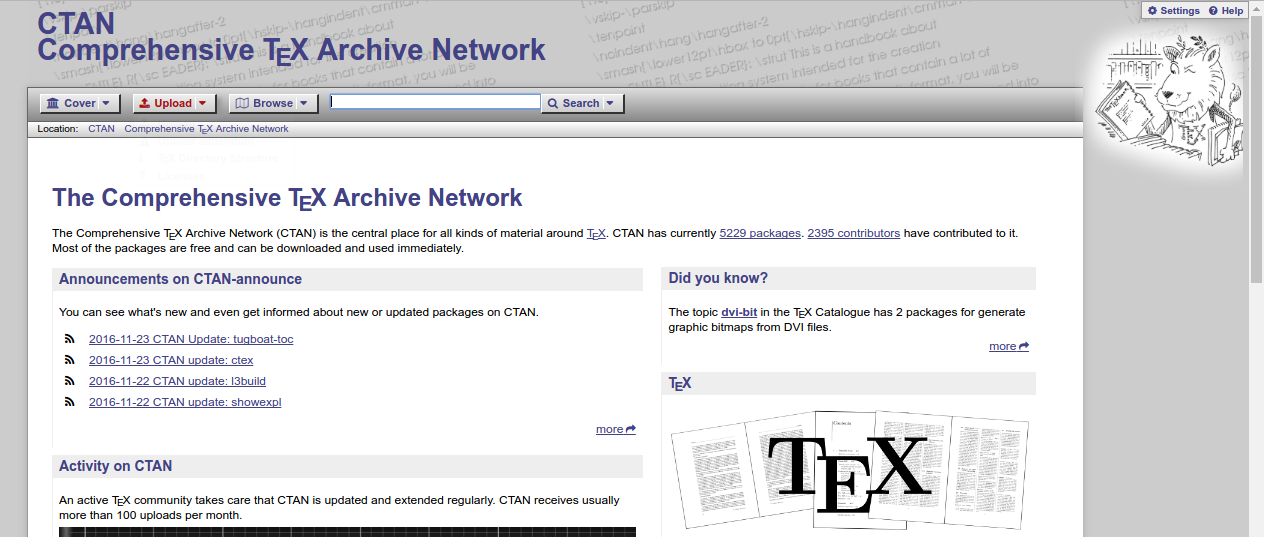
\includegraphics[width=0.7\linewidth]{CTAN.png}	
\end{frame}


\begin{frame}[fragile]
\frametitle{Хорошие мысли о \LaTeX!} 
\begin{itemize}
\item Каждый документ состоит из преамбулы и основной части;
\item Все \alert{комнады} начинаются с знака \verb|\|;
\item Аргументы команд стоят в фигурных скобках \{ \};
\item С помощью знака \% можно закомментировать какую-то часть документа, \LaTeX{} проигнорирует закомментированную часть;
\item Неважно сколько строк я оставил между абзацами и сколько пробелов я оставил между словами; 
\end{itemize}
\end{frame}

\section{Наш первый файл}
% Cоздаём первый файл до интеграла

\begin{frame}{Компиляция и её результаты}

\centering 
	\begin{tabulary}{\linewidth}{JcJ}
		\toprule
		  файл	  & & предназначение \\[0.25em]
		\midrule
		  .tex    & & мы пишем в этом файле  \\[0.25em]
		  .pdf    & & наш документ  \\[0.25em]
		  .log    & & логи, информация обо всём, что произошло во время компиляции  \\[0.25em]
		  .aux    & & карта документа, в нём записаны все ссылки, номера страниц, табоиц и т.д.  \\[0.25em]
          .synctex     & & позволяет нажать в pdf правую кнопку и перейти к соответствующему месту в tex-файле  \\[0.25em]
		\bottomrule
	\end{tabulary}
\end{frame}

\begin{frame}[fragile]
\frametitle{Формулы в \LaTeX!} 
\begin{itemize}
\item С помощью символа \$ мы можем перейти внутри текста в математический режим! Один \$ открывает математический режим, второй закрывает его!  \pause
\item С помощью символов \$\$ или \verb|\[| и \verb|\]| можно написать выключную формулу. Выключной объект --- такой объект, для которого необходима отдельная строка! \pause
\item Внутри математического режима \LaTeX{} сам расставляет пробелы. Все ваши пробелы игнорируются.
\end{itemize}
\end{frame}

% Смотрим кусок с интегралом!

\begin{frame}
\frametitle{Формулы в \LaTeX!} 
\begin{itemize}
\item В \LaTeX{} можно найти символы на все случаи жизни $\Im$
\item По {\color{blue} \href{http://detexify.kirelabs.org/classify.html}{этой ссылке}} расположен распознаватель символов! \pause
\item В книге Львовского есть огровное количество символов с подробными комментариями! Например: 
\centering  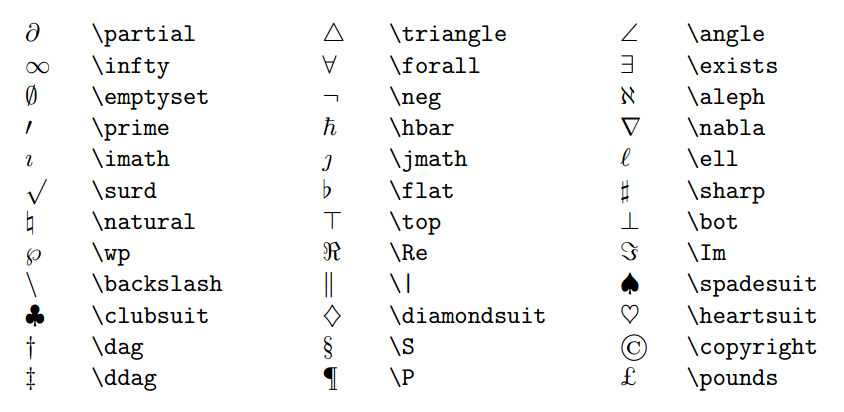
\includegraphics[scale=0.2]{table.png}
\end{itemize}
\end{frame}

% Распознать символ и вставить его

\begin{frame}
\frametitle{Служебные символы} 

\mbox{ } 

\centering
\Large{ \$ \% \{ \} \# \& — служебные символы}

\mbox{ }

\begin{itemize}
\item \normalsize{Чтобы использовать \$ или другой символ в тексте, надо написать $\setminus$\$.}
\end{itemize}
\end{frame}


\section{Подробнее о математике в \LaTeX{}} 


\section{Мотивация}

\begin{frame}{Мотивация}
	\centering
    \alert{\textbf{В \LaTeX{} никогда ничего никуда не съедет!}}
    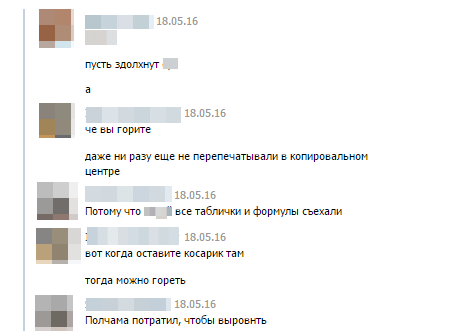
\includegraphics[height=0.68\textheight]{m1.png}
    
\end{frame}

\begin{frame}{Мотивация}
    \centering
    \alert{\textbf{В \LaTeX{} список литературы сгенерируется автоматически!}}
    
    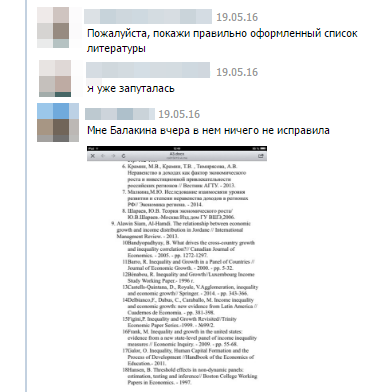
\includegraphics[height=0.68\textheight]{m2.png}
\end{frame}

\begin{frame}{Мотивация}
    \centering
    \alert{\textbf{Зачем первак, когда есть \LaTeX{}!}}
    
    
\includegraphics[height=0.68\textheight]{m4.png}
\end{frame}


\begin{frame}{Мотивация}
    \centering
    
\includegraphics[scale=0.5]{m5.png}
    
    \vfill
    \alert{\textbf{В \LaTeX{} можно написать абсолютно любой шаблон!}}
\end{frame}


\begin{frame}{Где раздобыть шаблоны}
\centering
\url{http://www.latextemplates.com/}

\includegraphics[width=0.6\linewidth]{template1.png}	

\url{https://www.overleaf.com/latex/templates}

\includegraphics[width=\linewidth]{template2.png}	
\end{frame}


\begin{frame}{Мотивация}
    \centering
    
\includegraphics[height=0.6\textheight]{m6.png}
    
    \vfill
    \alert{\textbf{В \LaTeX{} вы навсегда забудете о <<сначала энтер, потом 4 раза пробел>>!}}
\end{frame}


\begin{frame}{Мотивация}
    \centering
    
\includegraphics[scale=0.5]{m7.png}

	\mbox{ }     
     
    
\includegraphics[scale=0.6]{m9.png}
    
    \vfill
    \alert{\textbf{Проблемы при распечатке? Никогда не слышал!}}
\end{frame}


\begin{frame}{Мотивация}
    \centering
    
\includegraphics[scale=0.5]{m8.png}
    
    \vfill
    \alert{\textbf{В \LaTeX{} ничего не изменится и не исчезнет без вашего ведома!}}
\end{frame}


\begin{frame}{Мотивация}
    \centering
    
\includegraphics[scale=0.5]{m10.png}
    
    \vfill
    \alert{\textbf{А ещё то ли \LaTeX{} то ли ГОСТ придумали рептилоиды!}}
\end{frame}


\begin{frame}{А если говорить серьёзно, то \ldots} 
    \centering
    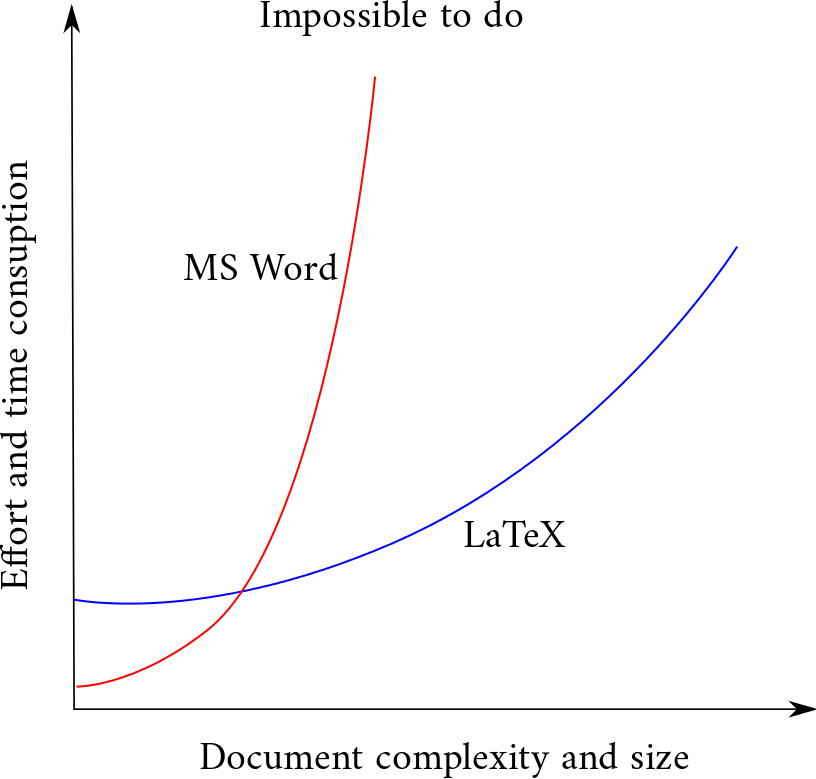
\includegraphics[scale=0.2]{latexvsword.png}
\end{frame}



\begin{frame}{Точка пересечения слишком близко}
\centering
    
\includegraphics[scale=0.48]{pain.png}


\url{http://www.kgasuclan.ru/blog/119-avtonumeracija-formul-risunkov-tablic-v-word.html}
\end{frame}


\section{Домашка} % Показать Pdf с домашкой, объяснить что делать!


\begingroup
\setbeamercolor{background canvas}{bg = LTXDarkGrey}
\begin{frame}[plain]
\vspace{0.5cm}
\centering \color{white}{\Huge{ KEEP CALM }}

\vspace{0.2cm}
\centering 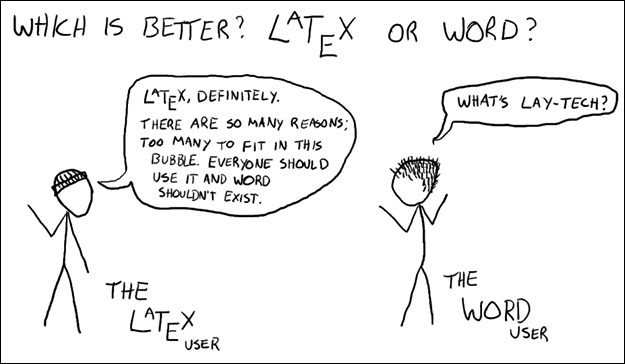
\includegraphics[width=0.8\linewidth]{joke_2.png}
\vspace{0.2cm}

\centering \color{white}{\Huge{ AND \TeX{ } IT }}
\end{frame}
\endgroup 

\end{document}

